\subsection{What is R?}
\makesubcontentsslidessec


\begin{frame}
  \begin{block}{What is R?}\pause
  \begin{minipage}{.75\textwidth}
  \begin{itemize}[<+-|alert@+>]
    \item \emph{lingua franca} for data analytics and statistical computing.
    \item Part programming language, part data analysis package.
  \end{itemize}
  \end{minipage}
  \hfill
  \begin{minipage}{.2\textwidth}
    \centering
\includegraphics[scale=2]{../common/pics/Rlogo}
  \end{minipage}
  \begin{itemize}
    \item Dialect of S (Bell Labs).
    \item Started May 5, 1976.
    \item Syntax designed for data.
  \end{itemize}
\end{block}
\end{frame}



\def\Put(#1,#2)#3{\leavevmode\makebox(0,0){\put(#1,#2){#3}}}
\begin{frame}
\vspace{-.1cm}
\begin{block}{Who uses R?}
\ \\[6.5cm]\ 
\end{block}
% top line
\Put(0,400){
\includegraphics[scale=1]{../common/pics/R_using_logos/oracle}}
\Put(135,410){
\includegraphics[scale=.1]{../common/pics/R_using_logos/merck}}
\Put(245,420){
\includegraphics[scale=.12]
  {../common/pics/R_using_logos/kickstarter}}
\Put(260,360){
\includegraphics[scale=.09]
  {../common/pics/R_using_logos/johndeere}}
%%%%
% second line
\Put(-5,315){
\includegraphics[scale=.2]{../common/pics/R_using_logos/boa}}
\Put(87,310){
\includegraphics[scale=.15]{../common/pics/R_using_logos/fb}}
\Put(145,355){
\includegraphics[scale=.12]{../common/pics/R_using_logos/ebay}}
\Put(135,270){
\includegraphics[scale=.9]{../common/pics/R_using_logos/mozilla}}
\Put(177,310){
\includegraphics[scale=.35]{../common/pics/R_using_logos/nyt}}
\Put(247,300){
\includegraphics[scale=.1]{../common/pics/R_using_logos/nist}}
%%%%
% third line
\Put(-50,210){
\includegraphics[scale=.05]{../common/pics/R_using_logos/shell}}
\Put(15,200){
\includegraphics[scale=.17]{../common/pics/R_using_logos/pfizer}}
\Put(92,188){
\includegraphics[scale=.22]{../common/pics/R_using_logos/fda}}
\Put(160,170){
\includegraphics[scale=.08]{../common/pics/R_using_logos/twitter}}
\Put(170,240){
\includegraphics[scale=.1]{../common/pics/R_using_logos/orbitz}}
\Put(250,250){
\includegraphics[scale=.12]{../common/pics/R_using_logos/cfpb}}
\Put(200,210){
\includegraphics[scale=.6]{../common/pics/R_using_logos/novartis}}
\Put(204,160){
\includegraphics[scale=.16]{../common/pics/R_using_logos/lloyds}}
%%%%
% fourth line
\Put(-50,90){
\includegraphics[scale=.12]{../common/pics/R_using_logos/google}}
\Put(50,130){
\includegraphics[scale=.12]{../common/pics/R_using_logos/bing}}
\Put(50,70){
\includegraphics[scale=.29]{../common/pics/R_using_logos/ford}}
\Put(140,80){
\includegraphics[scale=.25]{../common/pics/R_using_logos/zillow}}
\Put(215,80){
\includegraphics[scale=.15]{../common/pics/R_using_logos/okcupid}}
\end{frame}



% \begin{frame}
%   \begin{block}{Language Paradigms}\pause
%   \begin{center}
%     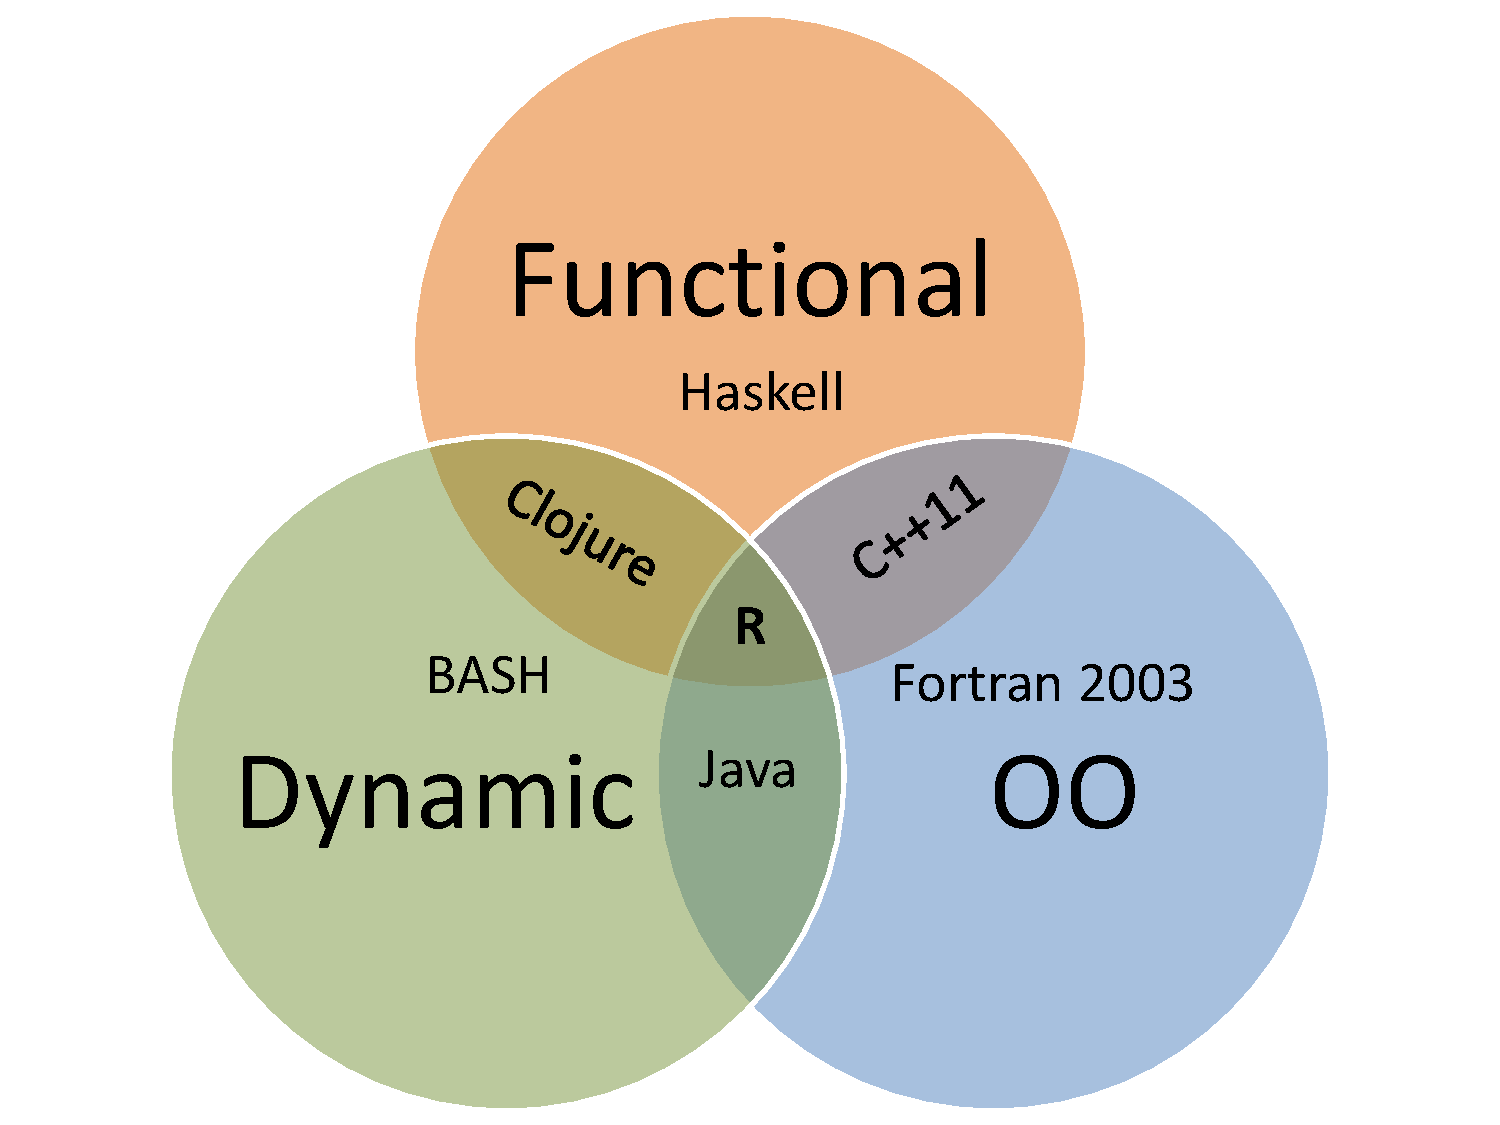
\includegraphics[scale=.35]{../common/pics/languages}
%   \end{center}
%   \end{block}
% \end{frame}


\begin{frame}
  \begin{block}{Resources to Learn R}\pause
  \begin{itemize}[<+-|alert@+>]
    \item \emph{Advanced R} by Hadley Wickham: \url{http://adv-r.had.co.nz/}
  \end{itemize}
\end{block}
\end{frame}